\newpage
\section{Dyson's Equation, Renormalization, RPA and Ladder Approximations}
\subsection{General types of partial sums}
\bgroup
\def\arraystretch{1.}
\begin{table}[H]
\begin{tabular}{cc}
\hline
General type of diagrams summed over                                                                                                                    & Result                                                                                                                            \\ \hline
\begin{tabular}[c]{@{}c@{}}(1) All diagrams containing repeated \\ proper (or 'irreducible') self-energy parts.\\  (Summation is complete)\end{tabular} & Dyson's equation                                                                                                                  \\ \hline
\begin{tabular}[c]{@{}c@{}}(2) All diagrams with "polarization\\  parts" inserted in interaction lines\end{tabular}                                     & \begin{tabular}[c]{@{}c@{}}"dressed", "effective" or\\ "renormalized" interactions\end{tabular}                                   \\\hline
\begin{tabular}[c]{@{}c@{}}(3) All diagrams with self-energy\\ parts' inserted in r ree particle\\ and bole lines\end{tabular}                          & \begin{tabular}[c]{@{}c@{}}"dressed" or "renormalized"\\ particle and bole lines (self-consistent\\ renormalization)\end{tabular} \\\hline
\begin{tabular}[c]{@{}c@{}}(4) All diagrams with 'irreducible\\ vertex parts' inserted in place of\\ a vertex\end{tabular}                              & dressed vertices     \\\hline                                     
\end{tabular}
\end{table}

\subsection{Dyson's Equation}
Let us first define "proper self-energy part" or "irreducible self-energy part". First we define:

\bluep{\textit{Self-energy part}}: Any diagram without incoming and outgoing lines, which can be inserted into a particle or hole line.

\bluep{\textit{Proper or irreducible self-energy part}}: A self-energy part which cannot be broken into two unconnected self-energy parts by removing one particle or hole line. Parts which can be so broken are called 'improper' or 'reducible'.

In general it is possible to sum over all repetitions of all irreducible self-energy parts in a diagram expansion:
\begin{equation}
    \includegraphics[width=0.8\textwidth]{screenshots/dyson-equation-1.PNG}
    \label{dyson-equation-1}
\end{equation}
or
\begin{equation}
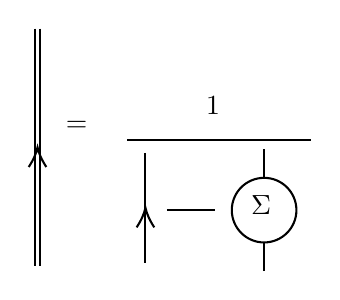
\begin{tikzpicture}[x=0.65pt,y=0.65pt,yscale=-1,xscale=1]
%uncomment if require: \path (0,300); %set diagram left start at 0, and has height of 300

%Straight Lines [id:da5007030956086185] 
\draw    (103.5,63.1) -- (103.5,195)(100.5,63.1) -- (100.5,195) ;
\draw [shift={(102,129.05)}, rotate = 90] [color={rgb, 255:red, 0; green, 0; blue, 0 }  ][line width=0.75]    (10.93,-4.9) .. controls (6.95,-2.3) and (3.31,-0.67) .. (0,0) .. controls (3.31,0.67) and (6.95,2.3) .. (10.93,4.9)   ;
%Straight Lines [id:da27166812193710055] 
\draw    (162,132.1) -- (162,193.1) ;
\draw [shift={(162,162.6)}, rotate = 90] [color={rgb, 255:red, 0; green, 0; blue, 0 }  ][line width=0.75]    (10.93,-4.9) .. controls (6.95,-2.3) and (3.31,-0.67) .. (0,0) .. controls (3.31,0.67) and (6.95,2.3) .. (10.93,4.9)   ;
%Straight Lines [id:da0814970714578146] 
\draw    (151.92,125.1) -- (253.92,125.1) ;
%Shape: Circle [id:dp3367153518929006] 
\draw   (210,163.96) .. controls (210,154.04) and (218.04,146) .. (227.96,146) .. controls (237.88,146) and (245.92,154.04) .. (245.92,163.96) .. controls (245.92,173.88) and (237.88,181.92) .. (227.96,181.92) .. controls (218.04,181.92) and (210,173.88) .. (210,163.96) -- cycle ;
%Straight Lines [id:da44172544983469675] 
\draw    (227.96,146) -- (227.96,130.1) ;
%Straight Lines [id:da9420867165019052] 
\draw    (227.96,197.82) -- (227.96,181.92) ;
%Straight Lines [id:da7785373748433801] 
\draw    (173.96,163.96) -- (200.92,163.96) ;

% Text Node
\draw (219,154) node [anchor=north west][inner sep=0.75pt]    {$\Sigma $};
% Text Node
\draw (194,99) node [anchor=north west][inner sep=0.75pt]    {$1$};
% Text Node
\draw (116,113) node [anchor=north west][inner sep=0.75pt]    {$=$};
\end{tikzpicture}
\label{dyson-eqn-2}
\end{equation}

Translated into functions this becomes:
\begin{equation}G(\mathbf{k}, \omega)=\frac{1}{\omega-\epsilon_{k}-\Sigma(\mathbf{k}, \omega)+i \delta_{k}}\end{equation}
where
\begin{equation}
    -i\Sigma(\mathbf{k},\omega)\equiv\Sigmapart
\end{equation}
It was necessary to restrict the sum to just repeated proper parts. If we had summed over repeated improper parts as well, diagrams would have been counted twice.

Equation (\ref{dyson-equation-1}) or (\ref{dyson-eqn-2}) is called \redp{Dyson's equation} and is the basic equation from which most propagator calculations start. $\Sigma(\mathbf{k},\omega)$ is a \textbf{\redp{generalized "effective field" or "effective potential" which the particle in state $\mathbf{k}$ sees because of its interaction with all the other particles of the system.}} This field is $\omega-$dependent, which describes the motion of the quasi-particle cloud in ($\mathbf{k},t$)-space.

\begin{imp}
The form of (\ref{dyson-eqn-2}) is only valid in the special cases of a system \redp{\textbf{with no external potential and with diagrams calculated in ($\mathbf{k},\omega$)-space.}} A more general form of the Dyson equation which holds whenever the single-particle propagator expansion holds:
\begin{equation}
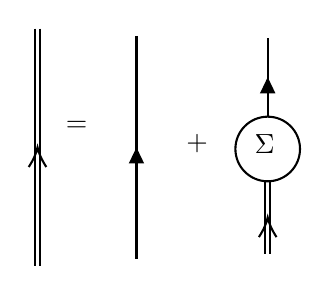
\begin{tikzpicture}[x=0.65pt,y=0.65pt,yscale=-1,xscale=1]
\draw    (103.5,63.1) -- (103.5,195)(100.5,63.1) -- (100.5,195) ;
\draw [shift={(102,129.05)}, rotate = 90] [color={rgb, 255:red, 0; green, 0; blue, 0 }  ][line width=0.75]    (10.93,-4.9) .. controls (6.95,-2.3) and (3.31,-0.67) .. (0,0) .. controls (3.31,0.67) and (6.95,2.3) .. (10.93,4.9)   ;
%Straight Lines [id:da27166812193710055] 
\draw    (157,67.1) -- (157,191.1) ;
\draw [shift={(157,129.1)}, rotate = 90] [fill={rgb, 255:red, 0; green, 0; blue, 0 }  ][line width=0.08]  [draw opacity=0] (8.93,-4.29) -- (0,0) -- (8.93,4.29) -- cycle    ;
%Shape: Circle [id:dp3367153518929006] 
\draw   (212,129.96) .. controls (212,120.04) and (220.04,112) .. (229.96,112) .. controls (239.88,112) and (247.92,120.04) .. (247.92,129.96) .. controls (247.92,139.88) and (239.88,147.92) .. (229.96,147.92) .. controls (220.04,147.92) and (212,139.88) .. (212,129.96) -- cycle ;
%Straight Lines [id:da44172544983469675] 
\draw    (229.96,112) -- (229.96,68.1) ;
\draw [shift={(229.96,90.05)}, rotate = 450] [fill={rgb, 255:red, 0; green, 0; blue, 0 }  ][line width=0.08]  [draw opacity=0] (8.93,-4.29) -- (0,0) -- (8.93,4.29) -- cycle    ;
%Straight Lines [id:da9420867165019052] 
\draw    (228.46,188.1) -- (228.46,147.92)(231.46,188.1) -- (231.46,147.92) ;
\draw [shift={(229.96,168.01)}, rotate = 450] [color={rgb, 255:red, 0; green, 0; blue, 0 }  ][line width=0.75]    (10.93,-4.9) .. controls (6.95,-2.3) and (3.31,-0.67) .. (0,0) .. controls (3.31,0.67) and (6.95,2.3) .. (10.93,4.9)   ;

% Text Node
\draw (221,120) node [anchor=north west][inner sep=0.75pt]    {$\Sigma $};
% Text Node
\draw (116,113) node [anchor=north west][inner sep=0.75pt]    {$=$};
% Text Node
\draw (183,120) node [anchor=north west][inner sep=0.75pt]    {$+$};


\end{tikzpicture}
\label{generalized-dyson-eqn}
\end{equation}
\end{imp}
Equation (\ref{generalized-dyson-eqn}) boils down to (\ref{dyson-eqn-2}) for a system without external potential because the value of each diagram is the product of the values of its parts:
\begin{equation}
   \tikzset{every picture/.style={line width=0.75pt}} %set default line width to 0.75pt        
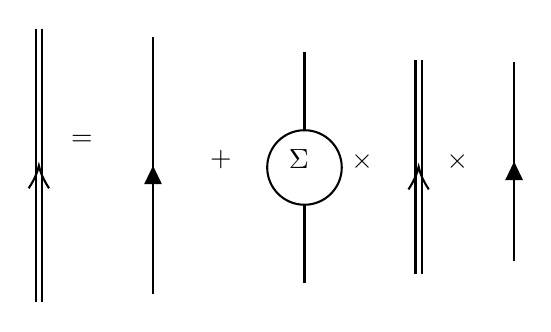
\begin{tikzpicture}[x=0.75pt,y=0.75pt,yscale=-1,xscale=1]
%uncomment if require: \path (0,300); %set diagram left start at 0, and has height of 300
\draw    (103.5,63.1) -- (103.5,195)(100.5,63.1) -- (100.5,195) ;
\draw [shift={(102,129.05)}, rotate = 90] [color={rgb, 255:red, 0; green, 0; blue, 0 }  ][line width=0.75]    (10.93,-4.9) .. controls (6.95,-2.3) and (3.31,-0.67) .. (0,0) .. controls (3.31,0.67) and (6.95,2.3) .. (10.93,4.9)   ;
%Straight Lines [id:da27166812193710055] 
\draw    (157,67.1) -- (157,191.1) ;
\draw [shift={(157,129.1)}, rotate = 90] [fill={rgb, 255:red, 0; green, 0; blue, 0 }  ][line width=0.08]  [draw opacity=0] (8.93,-4.29) -- (0,0) -- (8.93,4.29) -- cycle    ;
%Shape: Circle [id:dp3367153518929006] 
\draw   (212,129.96) .. controls (212,120.04) and (220.04,112) .. (229.96,112) .. controls (239.88,112) and (247.92,120.04) .. (247.92,129.96) .. controls (247.92,139.88) and (239.88,147.92) .. (229.96,147.92) .. controls (220.04,147.92) and (212,139.88) .. (212,129.96) -- cycle ;
%Straight Lines [id:da44172544983469675] 
\draw    (330.96,175.1) -- (330.96,79.1) ;
\draw [shift={(330.96,127.1)}, rotate = 450] [fill={rgb, 255:red, 0; green, 0; blue, 0 }  ][line width=0.08]  [draw opacity=0] (8.93,-4.29) -- (0,0) -- (8.93,4.29) -- cycle    ;
%Straight Lines [id:da9420867165019052] 
\draw    (283.46,181.1) -- (283.46,78.1)(286.46,181.1) -- (286.46,78.1) ;
\draw [shift={(284.96,129.6)}, rotate = 450] [color={rgb, 255:red, 0; green, 0; blue, 0 }  ][line width=0.75]    (10.93,-4.9) .. controls (6.95,-2.3) and (3.31,-0.67) .. (0,0) .. controls (3.31,0.67) and (6.95,2.3) .. (10.93,4.9)   ;
%Straight Lines [id:da9087104573290277] 
\draw    (229.96,74.1) -- (229.96,112) ;
%Straight Lines [id:da256765400607896] 
\draw    (229.96,147.92) -- (229.96,185.82) ;
\draw (221,120) node [anchor=north west][inner sep=0.75pt]    {$\Sigma $};
% Text Node
\draw (116,113) node [anchor=north west][inner sep=0.75pt]    {$=$};
% Text Node
\draw (183,120) node [anchor=north west][inner sep=0.75pt]    {$+$};
% Text Node
\draw (251,121) node [anchor=north west][inner sep=0.75pt]    {$\times $};
% Text Node
\draw (297,121) node [anchor=north west][inner sep=0.75pt]    {$\times $};


\end{tikzpicture} 
\end{equation}
or
\begin{equation}G(\mathbf{k}, \omega)=G_{0}(\mathbf{k}, \omega)+G(\mathbf{k}, \omega) \Sigma(\mathbf{k}, \omega) G_{0}(\mathbf{k}, \omega)\end{equation}
\redp{Equation (\ref{generalized-dyson-eqn}) is also valid when the diagrams do not factor}. For example, in $(\mathbf{k},t)$-space we find
\begin{equation}\begin{aligned}
i G\left(\mathbf{k}, t_{2}-t_{1}\right)=i &G_{0}\left(\mathbf{k}, t_{2}-t_{1}\right)+\\
&+\iint d t^{\prime} d t^{\prime \prime} i G_{0}\left(\mathbf{k}, t_{2}-t^{\prime \prime}\right)(-i) \Sigma\left(\mathbf{k}, t^{\prime \prime}-t^{\prime}\right) i G\left(\mathbf{k}, t^{\prime}-t_{1}\right)
\end{aligned}\end{equation}

Another example of (\ref{generalized-dyson-eqn}) is the case of a system with an external potential. Then
\begin{equation}\begin{aligned}
i G\left(k_{2}, k_{1} ; \omega\right)=i G_{0}&\left(k_{2}, \omega\right) \delta_{k_{2} k_{1}}+& \\
&+\sum_{k, k^{\prime}} i G_{0}\left(k_{2}, \omega\right) \delta_{k_{2} k^{\prime}}(-i) \Sigma\left(k^{\prime}, k ; \omega\right) i G\left(k, k_{1} ; \omega\right)
\end{aligned}\end{equation}
Note that now anomalous graphs must be included

\subsection{Quasi particles in low-density Fermi system (ladder approximation)}
We now describe the theory of Galitski for a system of particles interacting by means of short-range repulsive forces having range $a$, and with average distance between particles $r_0$. By 'low density' is meant that $a / r_{0} \ll 1 .$ This can also be stated in terms of $k_{F}$ since $n,$ the number of particles/cm $^{3}$ is equal to $\frac{1}{3} \pi^{-2} k_{F}^{3}$(\ref{N0-kF-relation}) and $n=1 / r_{0}^{3}$ so $1 / r_{0} \sim k_{F} .$ Hence the low-density criterion is that $k_{F} a \ll 1 .$ Such a theory can be applied in a qualitative way to the case of nuclear matter, where $a / r_{0} \sim \frac{1}{3},$ provided we neglect the attractive part of the nuclear potential.